\section*{Теоретическая часть:}
\begin{enumerate}
    \item Величины $n_o = \sqrt{\varepsilon_{\bot}}, n_e = \sqrt{\varepsilon_{\|}}$ называют главными показателями
преломления кристалла. \\
Выразим показатель преломления необыкновенной волны $n = \varepsilon$ через главные показатели преломления $n_o , n_e$ и угол между оптической осью и волновым вектором $\theta$:
\[ \frac{1}{n^2(\theta)} = \frac{\sin^2{\theta}}{n^2_e} + \frac{\cos^2{\theta}}{n^2_o} \]
Заметим, что при $\theta = \pi/2$ показатель преломления необыкновенной волны равен $n = n_e$, а при $\theta = 0$ он равен $n = n_o$. Для обыкновенной волны показатель преломления равен $n_o$ независимо от направления её распространения. \\
Если $n_o − n_e \ll n_o, n_e$ (для исландского шпата $n_o = 1,655, n_e = 1,485$
для $\lambda = 0,63$ мкм), формулу можно упростить:
\[ n(\theta) \approx n_e + (n_o - n_e) \cos^2{\theta}\]

\subsection*{Двойное лучепреломление в призме из исландского шпата.}
    \begin{figure}[h!]
    \centering
    \begin{subfigure}[b]{0.25\textwidth}
        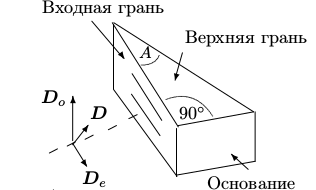
\includegraphics[width=\textwidth]{013.png}
    \end{subfigure}
    \begin{subfigure}[b]{0.25\textwidth}
        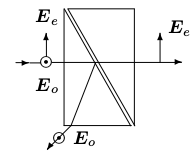
\includegraphics[width=\textwidth]{017.png}
    \end{subfigure}
    \caption\centering{а) Исследуемая призма из исландского шпата. Штриховкой указано направление оптической оси кристалла. б) Ход лучей в поляризационной призме}
    \end{figure}
    Значение показателя преломления и угол, под которым преломи-
лась волна в призме, можно найти, измерив угол падения на входную
грань призмы $\varphi_1$ и угол $\varphi_2$ на выходе призмы (рис. 2). Запишем закон Снеллиуса для одной из волн применительно к первой и второй граням призмы:
\[\sin{\varphi_1} = n \sin{\beta_1} \]
\[\sin{\varphi_2} = n \sin{\beta_2} = n \sin{(A - \beta_1)} \]
    \begin{figure}[h!]
        \noindent\centering{
            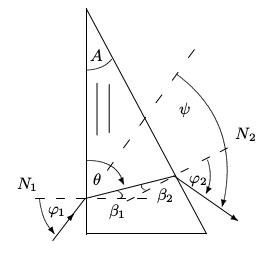
\includegraphics[height = 4cm]{018.png}
        }
        \caption{Ход лучей в призме}
    \end{figure}
    При этом мы выразили угол падения на вторую грань призмы $\beta_2$ через угол преломления на первой грани призмы $\beta_1$ и угол при вершине призмы $A$. Как видно из рис. 2, эти углы связаны простым соотношением: $A = \beta_1 + \beta_2$.\\
    Учитывая, что угол преломления $\beta_1$ связан с углом $\theta$ между осью кристалла и волновой нормалью $N$ соотношением $\theta + \beta_1 = \pi / 2$, находим $n$ и $\theta$:
\[ n = \frac{1}{\sin{A}} \sqrt{\sin^2{\varphi_1} + \sin^2{\varphi_2} + 2\sin{\varphi_1}\sin{\varphi_2}\cos{A} } \]
\[ \cos{A} = \frac{\sin{\varphi_1}}{n} \]    
    Для обыкновенной волны $n$ не будет зависеть от угла $\theta$, а для необыкновенной волны зависимость $n$ от $\theta$ должна описываться первой формулой. \\
    Показатель преломления призмы из изотропного материала удобно
находить по углу наименьшего отклонения луча от первоначального направления. Угол отклонения луча призмой ($\psi$ на рис. 2) минимален для симметричного хода лучей, т.е. когда $\varphi_1 = \varphi_2$ . Тогда показатель преломления можно рассчитать по формуле
\[n = \frac{\sin{\frac{\psi_m + A}{2}}}{\sin{\frac{A}{2}}} \]
где $\psi_m$ — угол наименьшего отклонения.    
\end{enumerate}